\documentclass{sig-alternate}
\usepackage{url}
\usepackage{graphicx}
\usepackage{subfigure}
\usepackage{hyperref}
\usepackage{url}
\usepackage{times}
\usepackage{balance}
\usepackage{xspace}
%\usepackage{xfrac}

\begin{document}

\newcommand{\todo}[1]{\textbf{TODO}\footnote{\textbf{TODO:} #1}}

\newcommand{\ghtorrent}{ \textsc{ght}orrent\xspace}
\newcommand{\api}{\textsc{api}\xspace}

\title{A dataset for pull-based development research}
\numberofauthors{3}

\author{
\alignauthor
Georgios Gousios\\
       \affaddr{Delft University of Technology}\\
       \affaddr{Delft, The Netherlands}\\
       \email{G.Gousios@tudelft.nl}
}

\maketitle

\begin{abstract}


\end{abstract}

\category{D.2.7}{Software Engineering}{Distribution, Maintenance, and Enhancement}[Version control]
\category{D.2.9}{Software Engineering}{Management}[Programming teams]

\terms{Management}

\keywords{pull-based development, pull request, distributed software development,
empirical software engineering}

\section{Introduction}
\label{sec:intro} 

\subsection{Data collection process}
\label{sec:expdata} 

After selection, the full history (including pull requests, issues and commits)
of the included projects was downloaded and features were extracted by querying
the {\sc ght}orrent databases and analyzing each project's Git repository. 
Furthermore, for these selected projects we collected all merges and the values for all factors that we use in our machine learning experiment, as described below.

\textbf{Merge detection.} To
identify merged pull requests that are merged outside Github, we resorted to the following heuristics, listed here in order of application:

\begin{enumerate}

  \item At least one of the commits associated with the pull request appears in
    the target project's master branch. 

  \item A commit closes the pull request (using the \texttt{fixes:} convention
    advocated by Github) and that commit appears in the project's master branch.
    This means that the pull request commits were squashed onto one commit and
    this commit was merged.

  \item One of the last 3 (in order of appearance) discussion comments contain a
    commit unique identifier, this commit appears in the project's master branch
    and the corresponding comment can be matched by the following regular
    expression:

    \begin{small}
    \texttt{(?:merg|appl|pull|push|integrat)(?:ing|i?ed)}
    \end{small}
  \item The latest comment prior to closing the pull request matches the 
    regular expression above.

\end{enumerate}

If none of the above heuristics identifies a merge, we mark the pull request
as unmerged. 

After creating the data files, we investigated projects where the pull request
merge ratio was significantly less than the one we calculated across Github
(73\%), and in any case less than 40\%, as this means that our heuristics are not
good enough for this project. This way, we filtered out 2 projects, which we did not
replace.

The final dataset consisted of 291 projects (99 Python, 91 Java, 87 Ruby, 14
Scala) and 166,884 pull requests (59,970; 55,468; 43,870 and 7,576 for Python,
Ruby, Java and Scala projects respectively). Both distributions are
representative of the contemporary popularity of each respective programming
language on both Github and other sites.

%Figure~\ref{fig:wordcloud} presents the project names in relative size to the
%pull requests included per project in the dataset. 
%
%\begin{figure}
%  \begin{center}
%    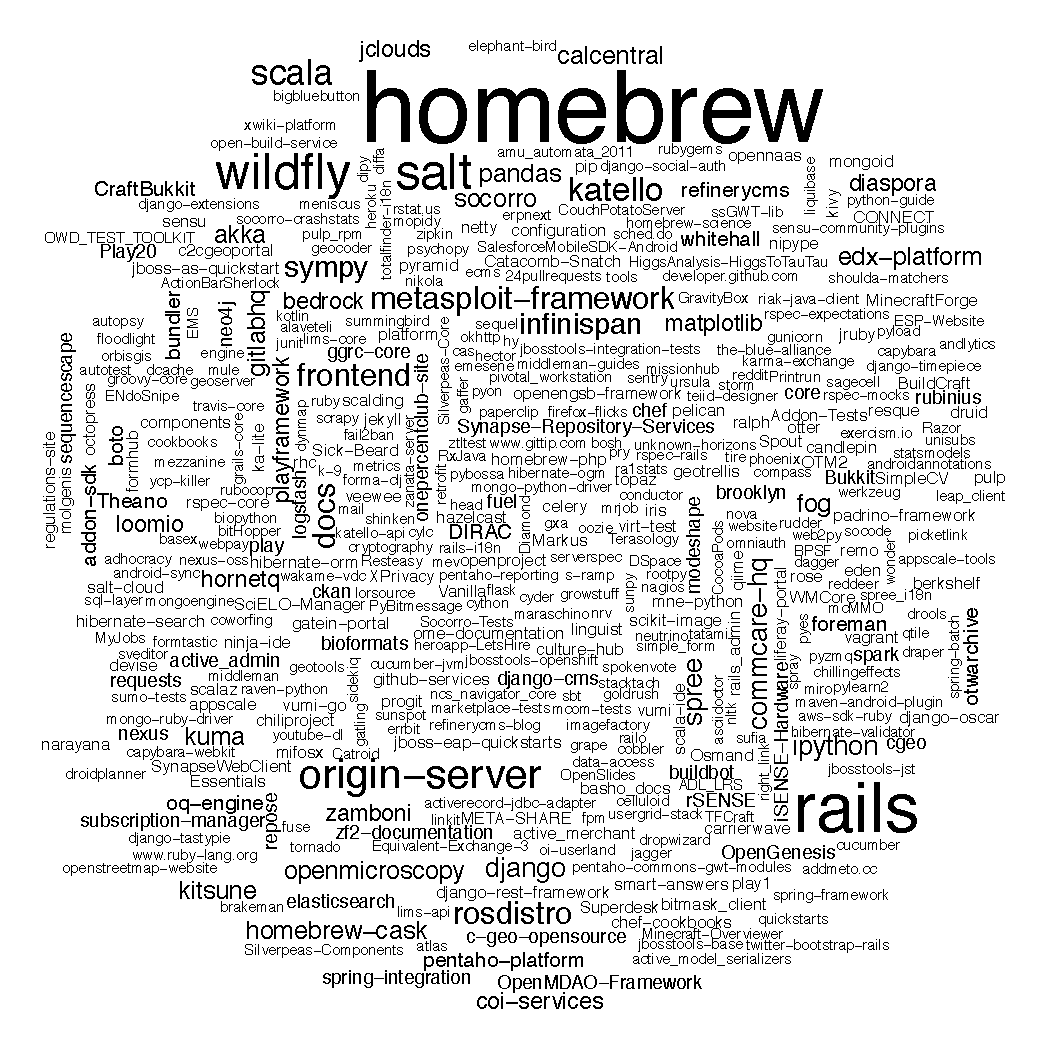
\includegraphics[scale=0.7]{wordcloud.pdf}
%  \end{center}
%  \caption{Projects in our dataset. Text size is relative to the number of
%  included pull requests.}
%  \label{fig:wordcloud}
%\end{figure}

\textbf{Feature Extraction.} The feature selection was based on prior work in the areas of patch submission and acceptance~\cite{Nagap05,Bird07a,Weiss08,Baysa12}, 
code reviewing~\cite{Rigby13}, bug
triaging~\cite{Anvik06, Giger10} and also on semi-structured interviews of
Github developers~\cite{Dabbi12, Pham13, McDon13}. The selected features are split
into three categories:

  \emph{Pull request characteristics.} These features attempt to quantify the
  impact of the pull request on the affected code base. When examining external
  code contributions, the size of the patch is affecting both acceptance and
  acceptance time~\cite{Weiss08}. There are various metrics to determine the
  size of a patch that have been used by researchers: code churn~\cite{Nagap05,
  Ratzi07}, changed files~\cite{Nagap05} and number of commits~\cite{Fluri07}.
  In the particular case of pull requests, developers reported that the presence
  of tests in a pull request increases their confidence to merge
  it~\cite{Pham13}. To investigate this, we split the churn feature into two
  features, namely \texttt{src\_churn} and \texttt{test\_churn}. The
  number of participants has been shown to influence the time to process of code
  reviewing~\cite{Rigby13}. Finally, through our own experience analyzing pull
  requests, we have found that in many cases conflicts are reported explicitly
  in pull request comments while in other cases pull requests include links to
  other related pull requests.

  \emph{Project characteristics.} These features quantify how receptive to pull
  requests the project is. If the project's process is open to external
  contributions, then we expect to see an increased ratio of external
  contributors over team members. The project's size may be a detrimental factor
  to the speed of processing a pull request, as its impact may be more difficult
  to assess. Also, incoming changes tend to cluster over time (the ``yesterday's
  weather'' change pattern~\cite{Girba04}), so it is natural to assume that pull
  requests affecting a part of the system that is under active development will
  be more likely to merge. Testing plays a role in speed of processing;
  according to~\cite{Pham13}, projects struggling with a constant flux of
  contributors use testing, manual or preferably automated, as a safety net to
  handle contributions from unknown developers.

  \emph{Developer.}  Developer-based features quantify the influence that the
  person who created the pull request has on the decision to merge it and the
  time to process it. In particular, the developer who created the patch has
  been shown to influence the patch acceptance decision~\cite{Jeong09}. To
  abstract the results across projects with different developers, we include
  features that quantify the developer's track record~\cite{Dabbi12}, namely the
  number of previous pull requests and their acceptance rate; the former has
  been identified as a strong indicator of pull request quality~\cite{Pham13}.
  Bird et al.~\cite{Bird07}, presented evidence that social reputation has an
  impact on whether a patch will be merged; in our dataset, the number of
  followers on Github can be seen as a proxy for reputation.

All features are calculated at the time a pull request has been closed or
merged, to evaluate the effect of intermediate updates to the pull request as a
result of the ensuing discussion. Features that contain a temporal dimension in
their calculation (e.g., \texttt{team\_size} or
\texttt{commits\_on\_files\_touched}) are calculated over the three-month time
period before the pull request was opened.

% latex table generated in R 2.15.3 by xtable 1.7-1 package
% Sat Jan 11 16:56:59 2014
\begin{table*}
\centering
\begin{tabular}{rp{20em}rrrrc}
  \hline
  \bfseries{Feature} & \bfseries{Description} & \bfseries{5\%} & \bfseries{mean} & \bfseries{median} & \bfseries{95\%} & \bfseries{histogram} \\ 
  \hline
   \multicolumn{2}{l}{\bf{Pull Request Characteristics}}\\
lifetime\_minutes & Minutes between opening and closing & 0.00 & 15,418 & 581.00 & 72,508 & 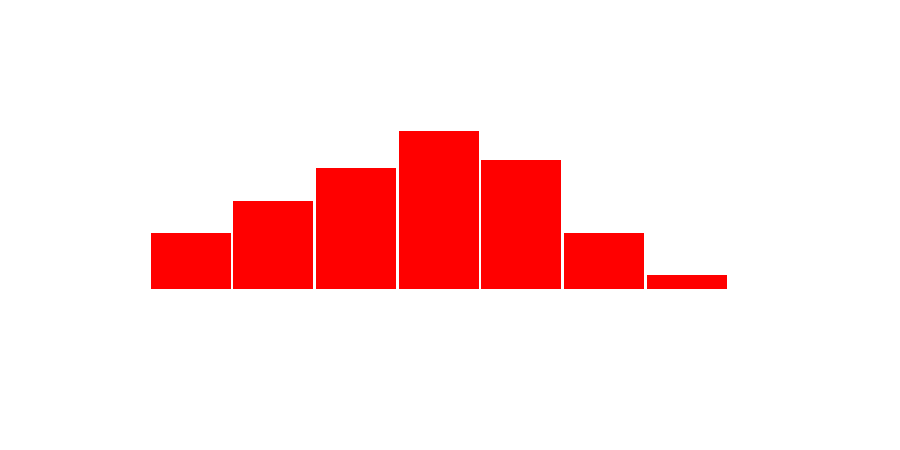
\includegraphics[scale = 0.1, clip = true, trim= 50px 60px 50px 60px]{hist-29b6fa715eecc1dad108c8148465533b.pdf} \\ 
  mergetime\_minutes & Minutes between opening and merging (only for merged pull
    requests) & 0.00 & 10,506 & 418.00 & 44,234 & 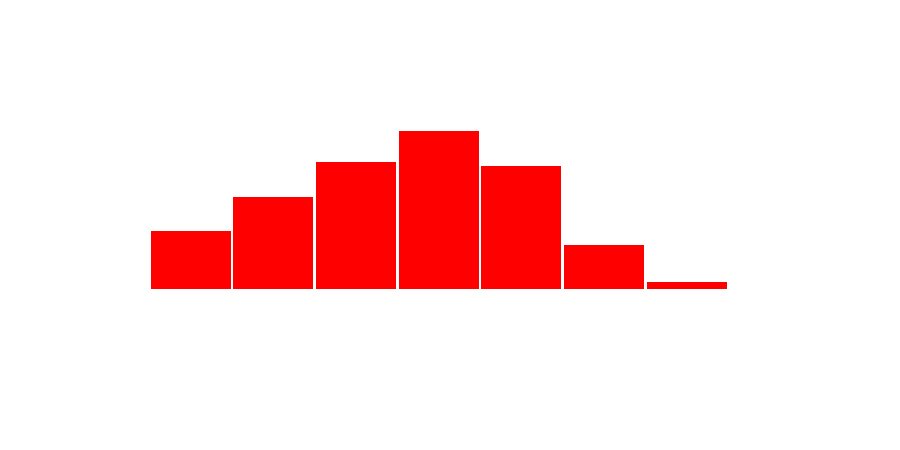
\includegraphics[scale = 0.1, clip = true, trim= 50px 60px 50px 60px]{hist-e2ded77f4080f561e112a1f363b125ce.pdf} \\ 
  num\_commits & Number of commits & 1.00 & 4.42 & 1.00 & 12.00 & 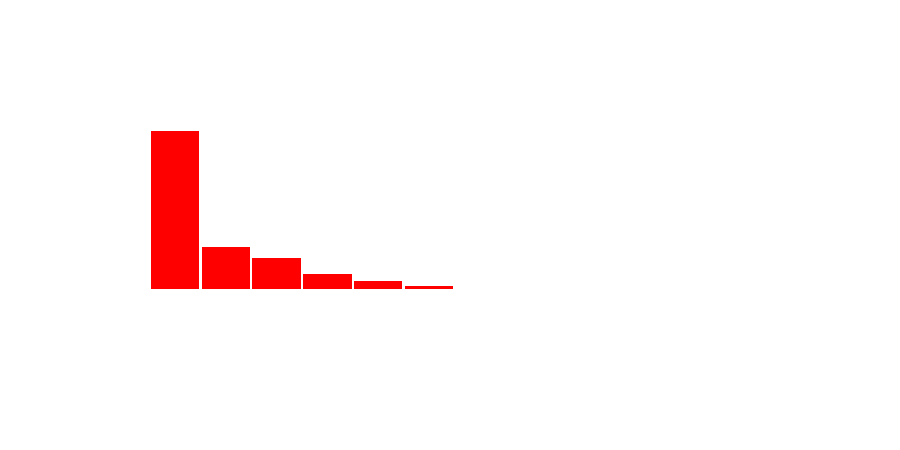
\includegraphics[scale = 0.1, clip = true, trim= 50px 60px 50px 60px]{hist-f128f3cb38588fe5202716588c047381.pdf} \\ 
  src\_churn & Number of lines changed (added + deleted) & 0.00 & 282.95 & 10.00 & 846.00 & 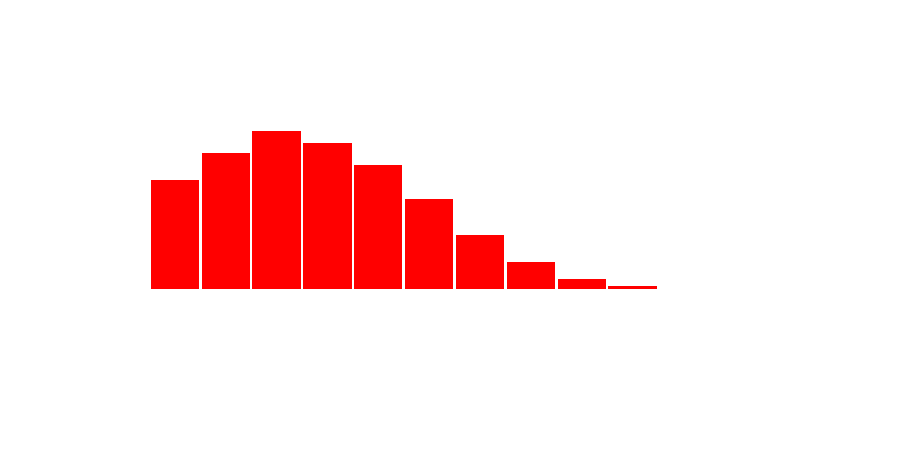
\includegraphics[scale = 0.1, clip = true, trim= 50px 60px 50px 60px]{hist-1f006c80a0da61518435a0c55f538326.pdf} \\ 
  test\_churn & Number of test lines changed & 0.00 & 79.74 & 0.00 & 248.00 & 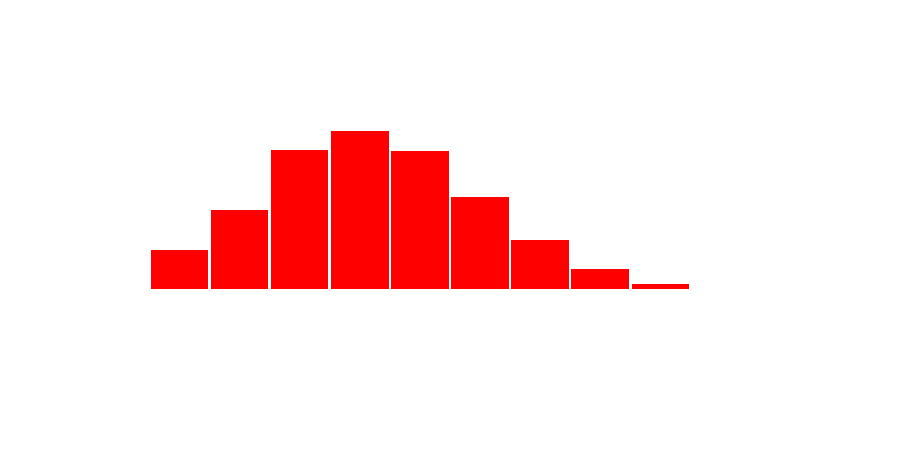
\includegraphics[scale = 0.1, clip = true, trim= 50px 60px 50px 60px]{hist-dd78ccaeedd7fc79735a66eb7f9e506b.pdf} \\ 
  files\_added & Number of files added  & 0.00 & 4.01 & 0.00 & 7.00 & 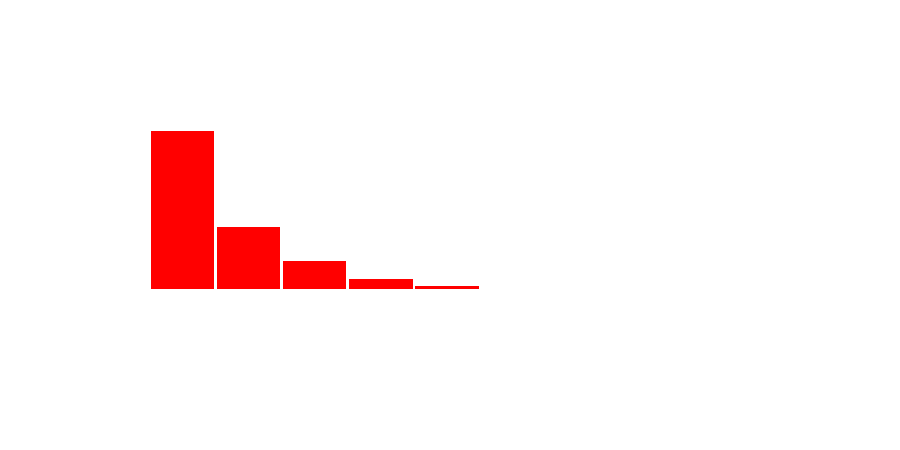
\includegraphics[scale = 0.1, clip = true, trim= 50px 60px 50px 60px]{hist-340be33adc9a51666460c68028842c1d.pdf} \\ 
  files\_deleted & Number of files deleted  & 0.00 & 2.05 & 0.00 & 1.00 & \includegraphics[scale = 0.1, clip = true, trim= 50px 60px 50px 60px]{hist-bd564691a0c6275ea5f30bcc0b81b3f5.pdf} \\ 
  files\_modified & Number of files modified  & 1.00 & 7.56 & 2.00 & 21.00 & 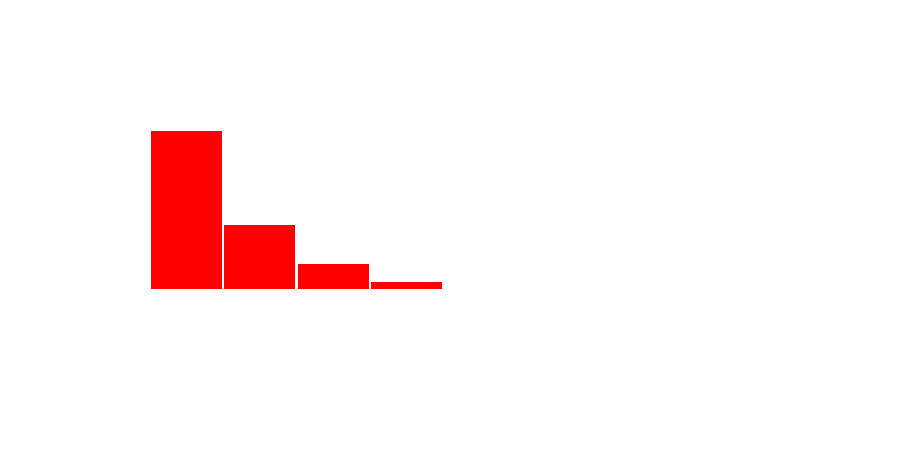
\includegraphics[scale = 0.1, clip = true, trim= 50px 60px 50px 60px]{hist-52a19dc5ca5e4f8c5325bca43137a6c1.pdf} \\ 
  files\_changed & Number of files touched (sum of the above) & 1.00 & 13.62 & 2.00 & 32.00 & 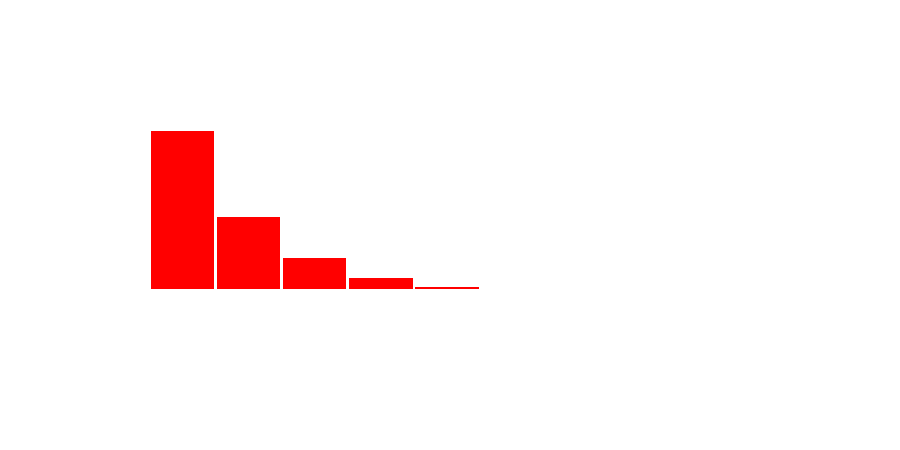
\includegraphics[scale = 0.1, clip = true, trim= 50px 60px 50px 60px]{hist-9b07b060359435635ff2bf4cd34f834a.pdf} \\ 
  src\_files & Number of source code files touched by the pull request & 0.00 & 7.64 & 1.00 & 20.00 & 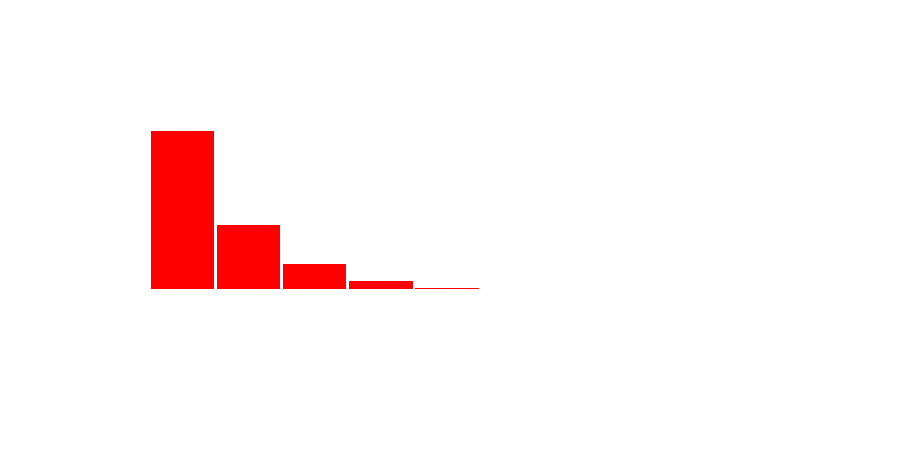
\includegraphics[scale = 0.1, clip = true, trim= 50px 60px 50px 60px]{hist-2d4e53ba8eec29c0c79c1e834756c654.pdf} \\ 
  doc\_files & Number of documentation (markup) files touched & 0.00 & 2.36 & 0.00 & 6.00 & 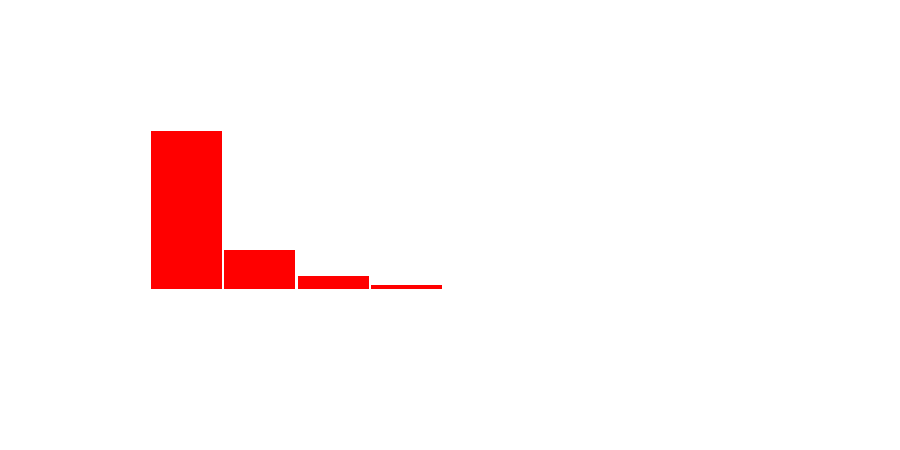
\includegraphics[scale = 0.1, clip = true, trim= 50px 60px 50px 60px]{hist-d4fb585969e7acb86dd568d80e7f1500.pdf} \\ 
  other\_files & Number of non-source, non-documentation files touched & 0.00 & 2.74 & 0.00 & 4.00 & 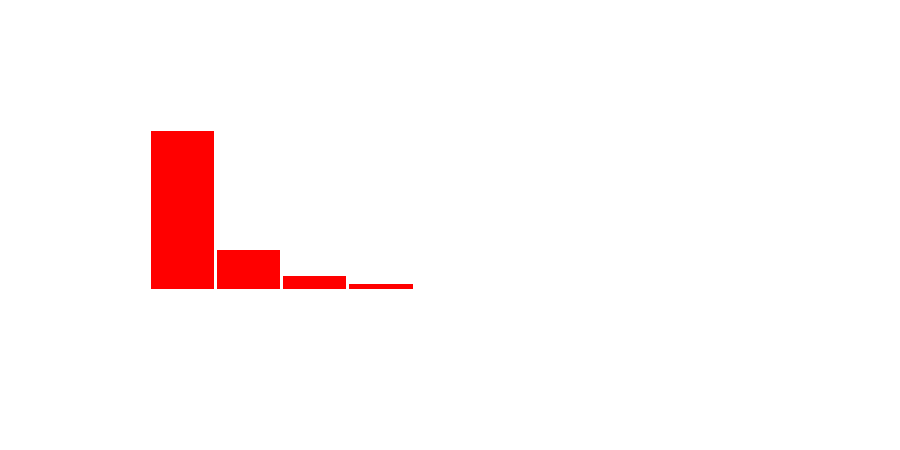
\includegraphics[scale = 0.1, clip = true, trim= 50px 60px 50px 60px]{hist-df965fcd0b03a96f1b31b2eda13d2b98.pdf} \\ 
  num\_commit\_comments & The total number of code review comments & 0.00 & 0.73 & 0.00 & 4.00 & 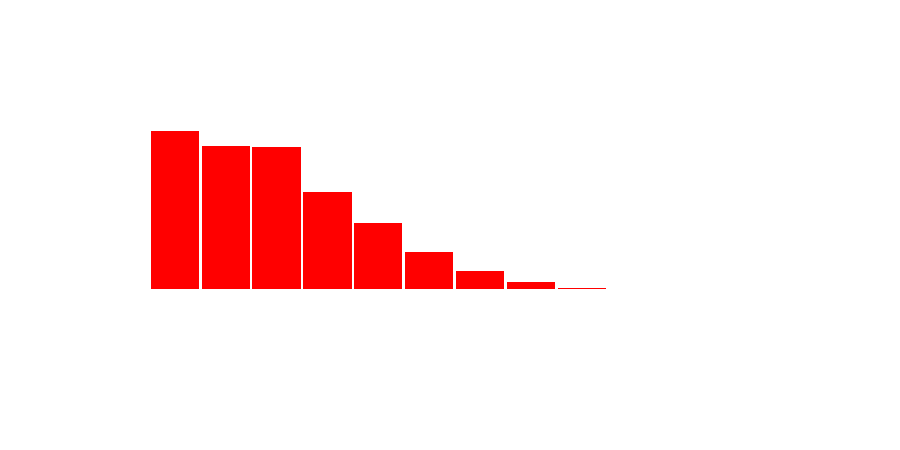
\includegraphics[scale = 0.1, clip = true, trim= 50px 60px 50px 60px]{hist-f0fac61db5a83629be8f04cc84e8b907.pdf} \\ 
  num\_issue\_comments & The total number of discussion comments & 0.00 & 1.84 & 0.00 & 8.00 & 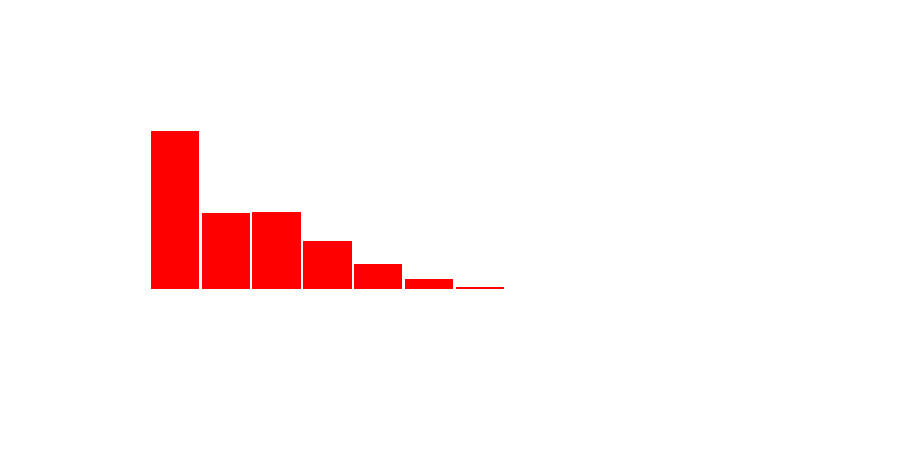
\includegraphics[scale = 0.1, clip = true, trim= 50px 60px 50px 60px]{hist-fee6653ed7b2359f7e7374841378492b.pdf} \\ 
  num\_comments & The total number of comments (discussion and code review). & 0.00 & 2.57 & 1.00 & 11.00 & 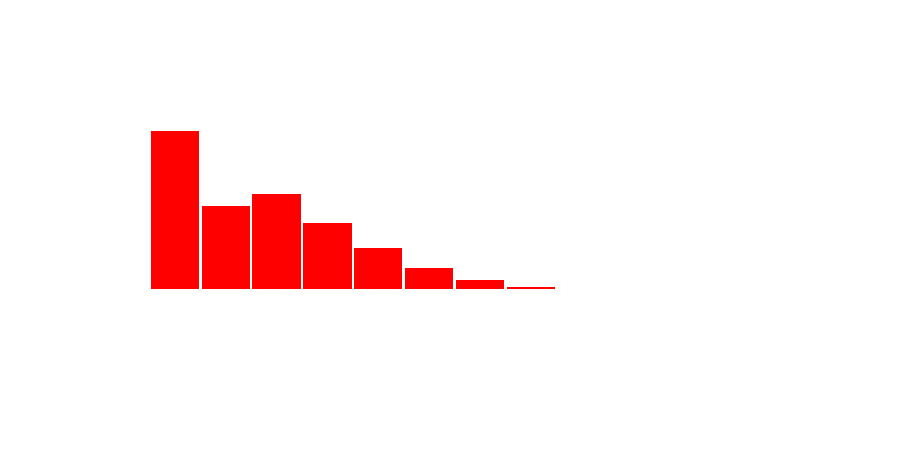
\includegraphics[scale = 0.1, clip = true, trim= 50px 60px 50px 60px]{hist-9db5e2b390de0d64d26c14798cb579ef.pdf} \\ 
  num\_participants & Number of participants in the discussion & 0.00 & 1.27 & 1.00 & 4.00 & 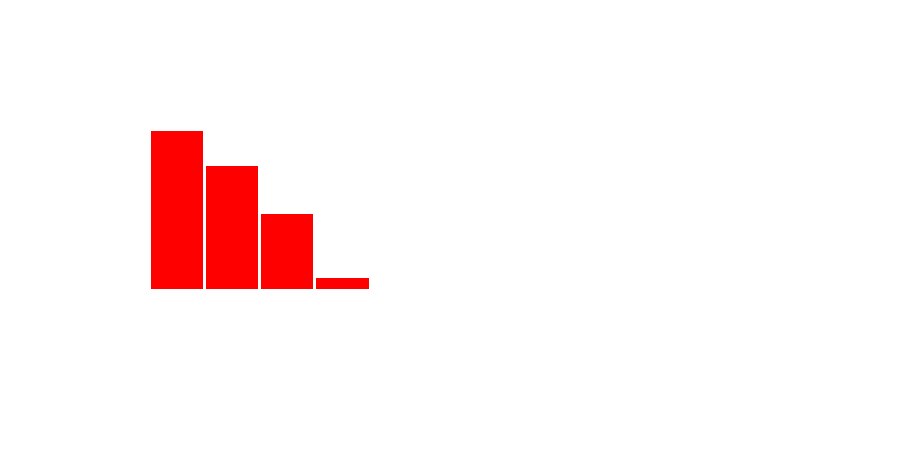
\includegraphics[scale = 0.1, clip = true, trim= 50px 60px 50px 60px]{hist-7d419bb69f175ea7015a9bdc71172f38.pdf} \\ 
  \multicolumn{2}{l}{\bf{Project Characteristics}}\\
  
  sloc & Executable lines of code at creation time. & 458.00 & 53,801 & 18,019 & 275,058 & 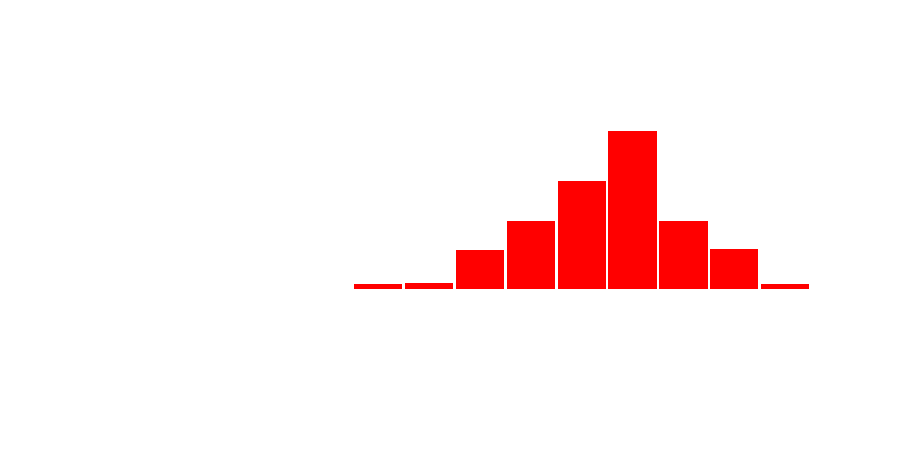
\includegraphics[scale = 0.1, clip = true, trim= 50px 60px 50px 60px]{hist-6b5159d3060b4fdf8493d4c818f79949.pdf} \\ 
  team\_size & Number of active core team members during the last 3 months prior to creation. & 1.00 & 20.64 & 7.00 & 93.00 & 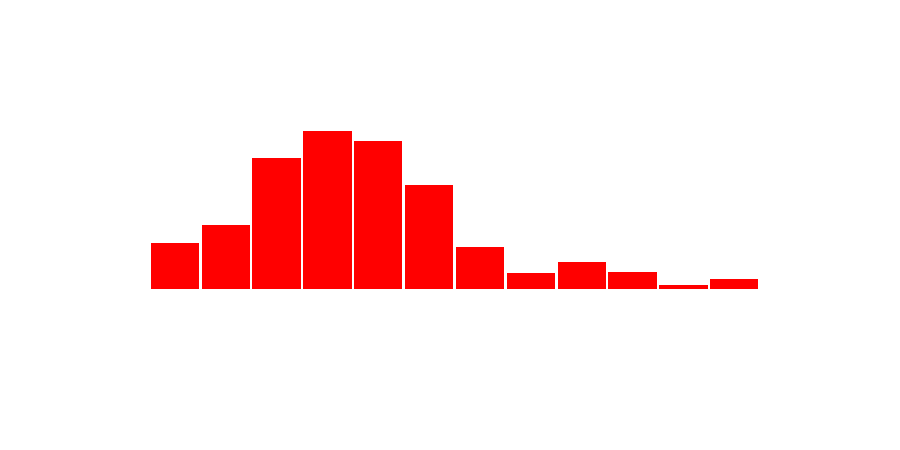
\includegraphics[scale = 0.1, clip = true, trim= 50px 60px 50px 60px]{hist-231fb4fabf4a3f0c551f2a97ae080508.pdf} \\ 
  perc\_external\_contribs & The ratio of commits from external members over core team members in the last 3 months prior to creation. & 8.00 & 54.01 & 56.00 & 95.00 & 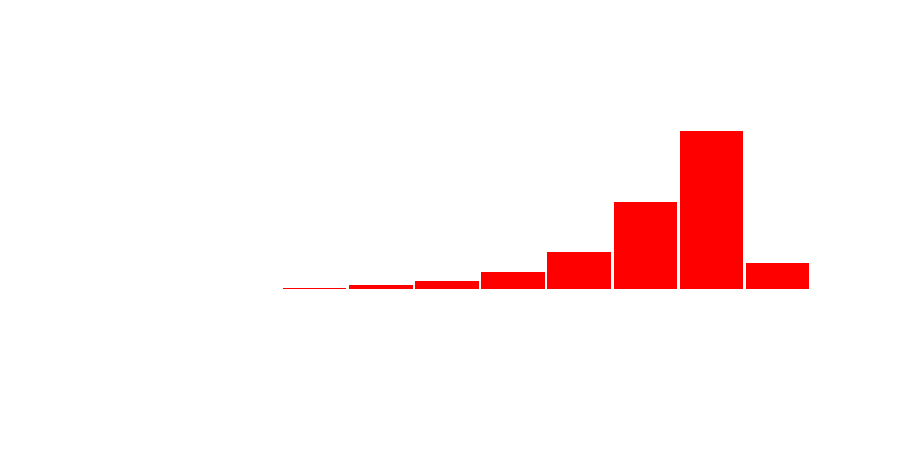
\includegraphics[scale = 0.1, clip = true, trim= 50px 60px 50px 60px]{hist-a222f0a5c377ba129dd6c8f257062591.pdf} \\ 
  commits\_on\_files\_touched & Number of total commits on files touched by the pull request 3 months before the creation time. & 0.00 & 51.65 & 4.00 & 209.00 & 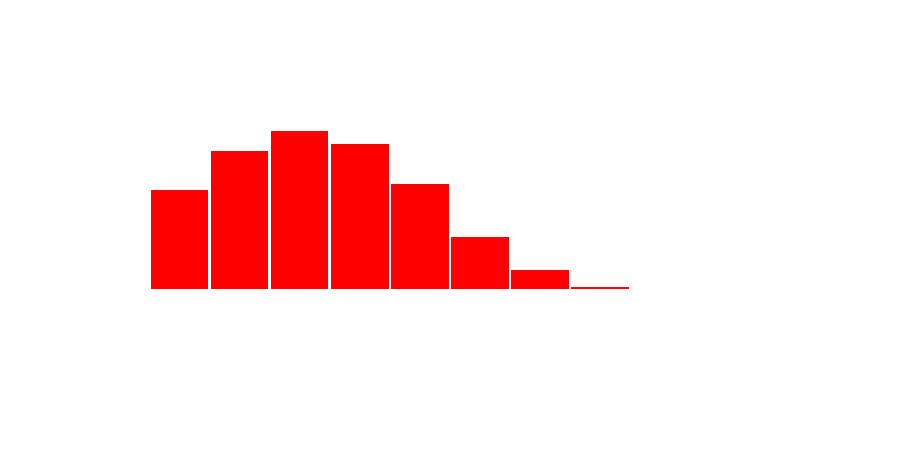
\includegraphics[scale = 0.1, clip = true, trim= 50px 60px 50px 60px]{hist-b735900ffcc37e7eda16dcd0c3497e6e.pdf} \\ 
  test\_lines\_per\_kloc & Executable lines of test code per 1,000 lines of source code & 0.00 & 1,297 & 355.21 & 2,097 & 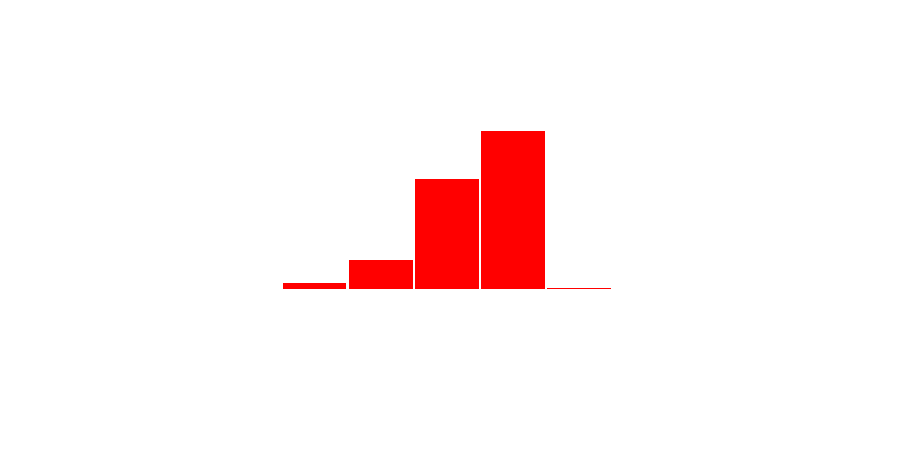
\includegraphics[scale = 0.1, clip = true, trim= 50px 60px 50px 60px]{hist-67ff3047089ba9ce0528884eab66e80a.pdf} \\ 
  test\_cases\_per\_kloc & Number of test cases per 1,000 lines of source code & 0.00 & 83.74 & 14.55 & 181.03 & 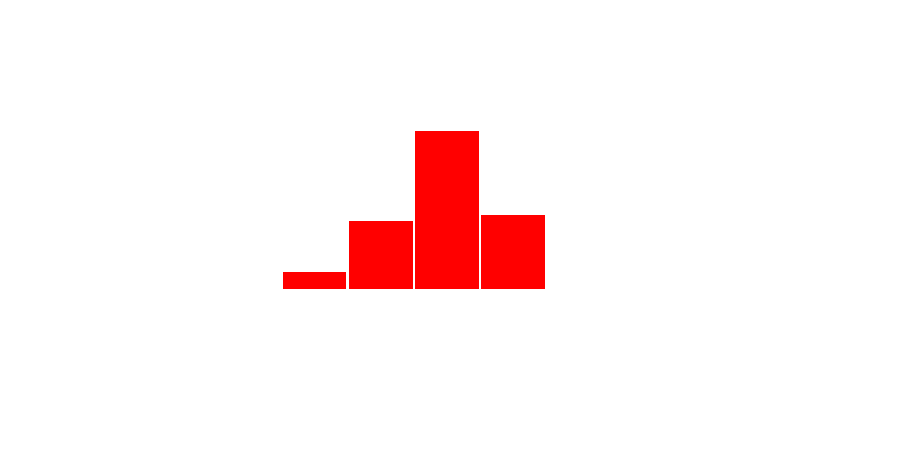
\includegraphics[scale = 0.1, clip = true, trim= 50px 60px 50px 60px]{hist-2b62bb5f7ccb31fe66208a895c8dd549.pdf} \\ 
  asserts\_per\_kloc & Number of assert statements per 1,000 lines of source code & 0.00 & 200.30 & 40.37 & 479.11 & 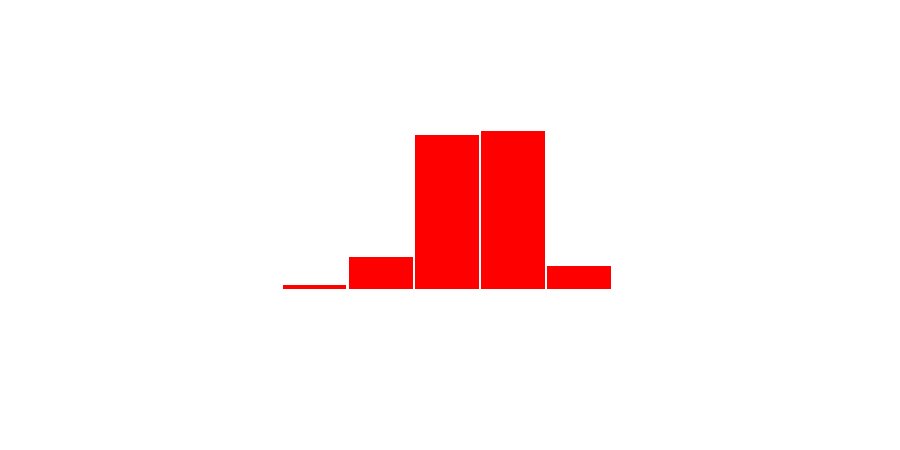
\includegraphics[scale = 0.1, clip = true, trim= 50px 60px 50px 60px]{hist-4ad84a89acf32483001ce11c881622b8.pdf} \\ 
  watchers & Project watchers (stars) at creation & 4.00 & 1,778 & 310.00 & 11,114 & 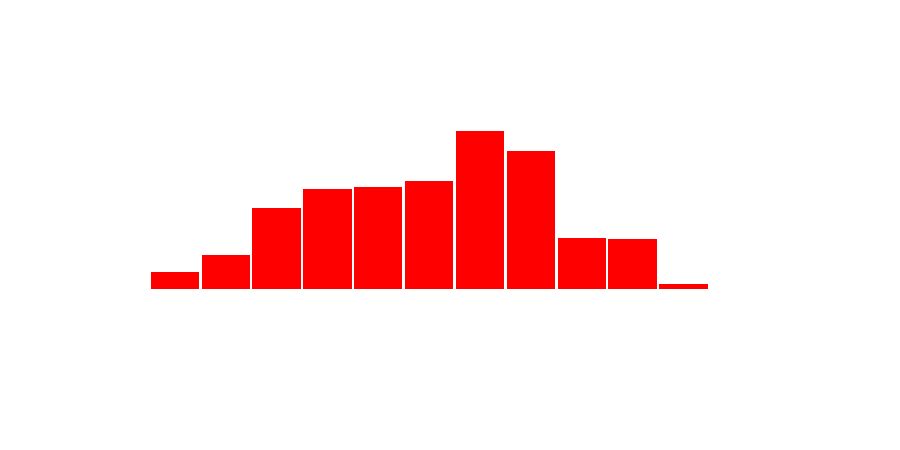
\includegraphics[scale = 0.1, clip = true, trim= 50px 60px 50px 60px]{hist-d097a7d1786ca9917e46e0fda1adb365.pdf} \\

  \multicolumn{2}{l}{\bf{Developer Characteristics}}\\
  
  prev\_pullreqs & Number of pull requests submitted by a specific developer, prior to the examined one & 0.00 & 42.81 & 11.00 & 196.00 & 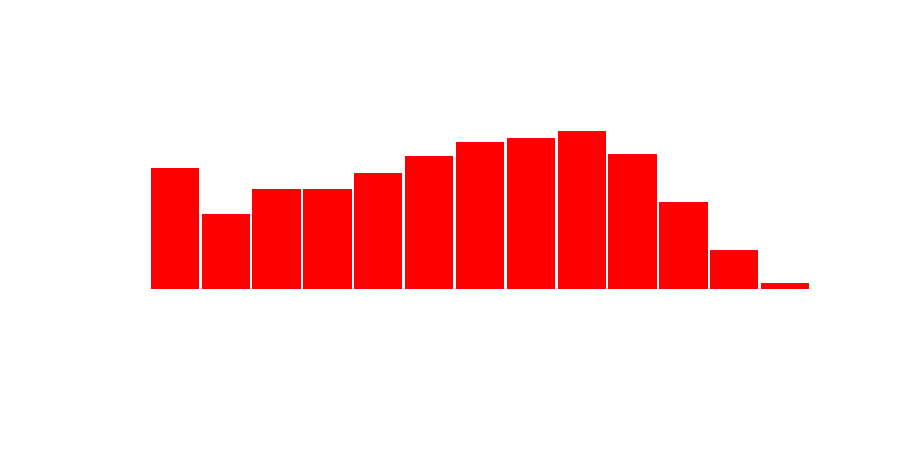
\includegraphics[scale = 0.1, clip = true, trim= 50px 60px 50px 60px]{hist-a2f7f60851dfa13cfbe0227d1d233767.pdf} \\ 
  requester\_succ\_rate & The percentage of the developer's pull requests that have been merged up to the creation of the examined one & 0.00 & 0.51 & 0.62 & 1.00 & 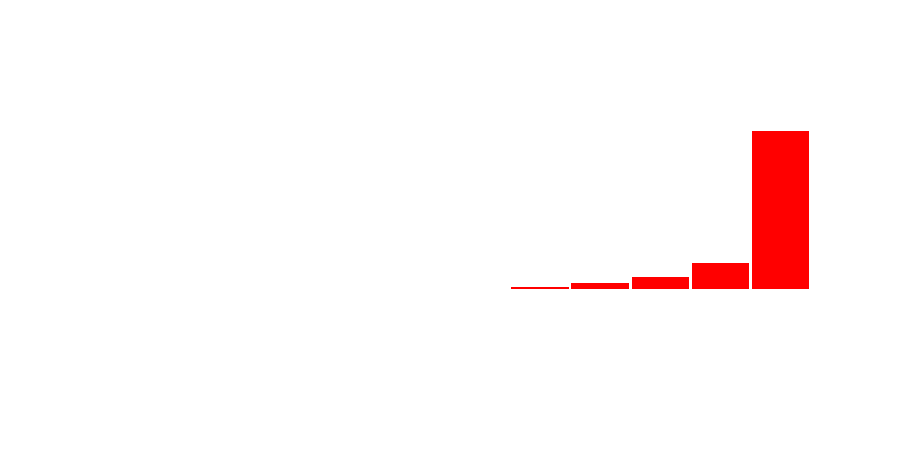
\includegraphics[scale = 0.1, clip = true, trim= 50px 60px 50px 60px]{hist-9363017165c3ded62457750f1c67c1af.pdf} \\ 
  followers & Followers to the developer at creation & 0.00 & 20.93 & 4.00 & 80.00 & 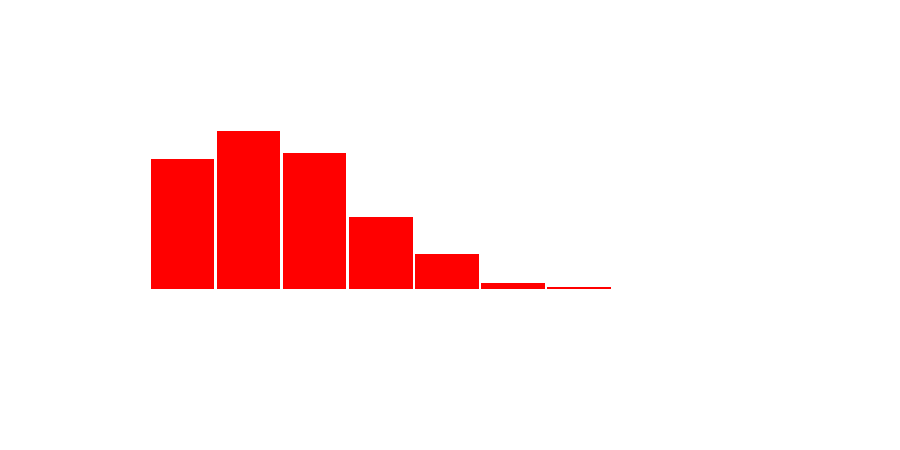
\includegraphics[scale = 0.1, clip = true, trim= 50px 60px 50px 60px]{hist-a7f2f738f15a09420e70e9a2c30e2aef.pdf} \\ 
   \hline
\end{tabular}
\caption{Selected features and descriptive statistics. A data point is a pull request. Historgrams are in log scale.} 
\label{tab:features}
\end{table*}


\section{Challenges and limitations}
\label{sec:challenges}

\paragraph*{Merge detection is incomplete}

\paragraph*{Projects are incomplete}

\paragraph*{Test detection is approximate}


\section{Research opportunities}
\label{sec:discussion}

\section{Related Work}
\label{sec:rel}


\section{Conclusion}

%\subsection*{Acknowledgements}

%We would like to thank the anonymous reviewers for their comments.
%This work is partially supported by Marie Curie {\sc ief} 298930 --- {\sc sefunc}.

\bibliographystyle{abbrv}
\balance
%\begin{small}

  \bibliography{dataset}
%\end{small}

\end{document}
